% The contents of this file is 
% Copyright (c) 2009-  Charles R. Severance, All Righs Reserved

\chapter{Uso de servicios web}

Una vez que recuperar documentos a través de HTTP y analizarlos usando
programas se convirtió en algo sencillo,
no se tardó demasiado en desarrollar un modelo
consistente en la producción de
documentos específicamente diseñados para ser consumidos por otros
programas (es decir, no sólo HTML para ser mostrado en un navegador).

Existen dos formatos habituales que se usan para intercambio de datos a través de la web.
El ``eXtensible Markup Language (lenguaje extensible de marcas)'' o XML ha sido utilizado
durante mucho tiempo y es el más adecuado para intercambiar datos del tipo-documento.
Cuando los programas simplemente quieren intercambiar unos con otros diccionarios, listas u otra
información interna, usan JavaScript Object Notation (Notación de Objetos Javascript), o JSON
(see \url{www.json.org}). Nosotros vamos a revisar ambos formatos.

\section{eXtensible Markup Language - XML}

XML tiene un aspecto muy parecido a HTML, pero XML está más estructurado.
Esto es un ejemplo de un documento XML:

\beforeverb
\begin{verbatim}
<persona>
  <nombre>Chuck</nombre>
  <telefono tipo="intl">
     +1 734 303 4456
   </telefono>
   <email oculto="si"/>
</persona>
\end{verbatim}
\afterverb
%
A veces resulta útil pensar en un documento XML como en la estructura de un árbol,
donde hay una etiqueta superior {\tt persona}, y otras etiquetas como {\tt telefono}
que se dibujan como \emph{hijas} de sus nodos padres.

\beforefig
\centerline{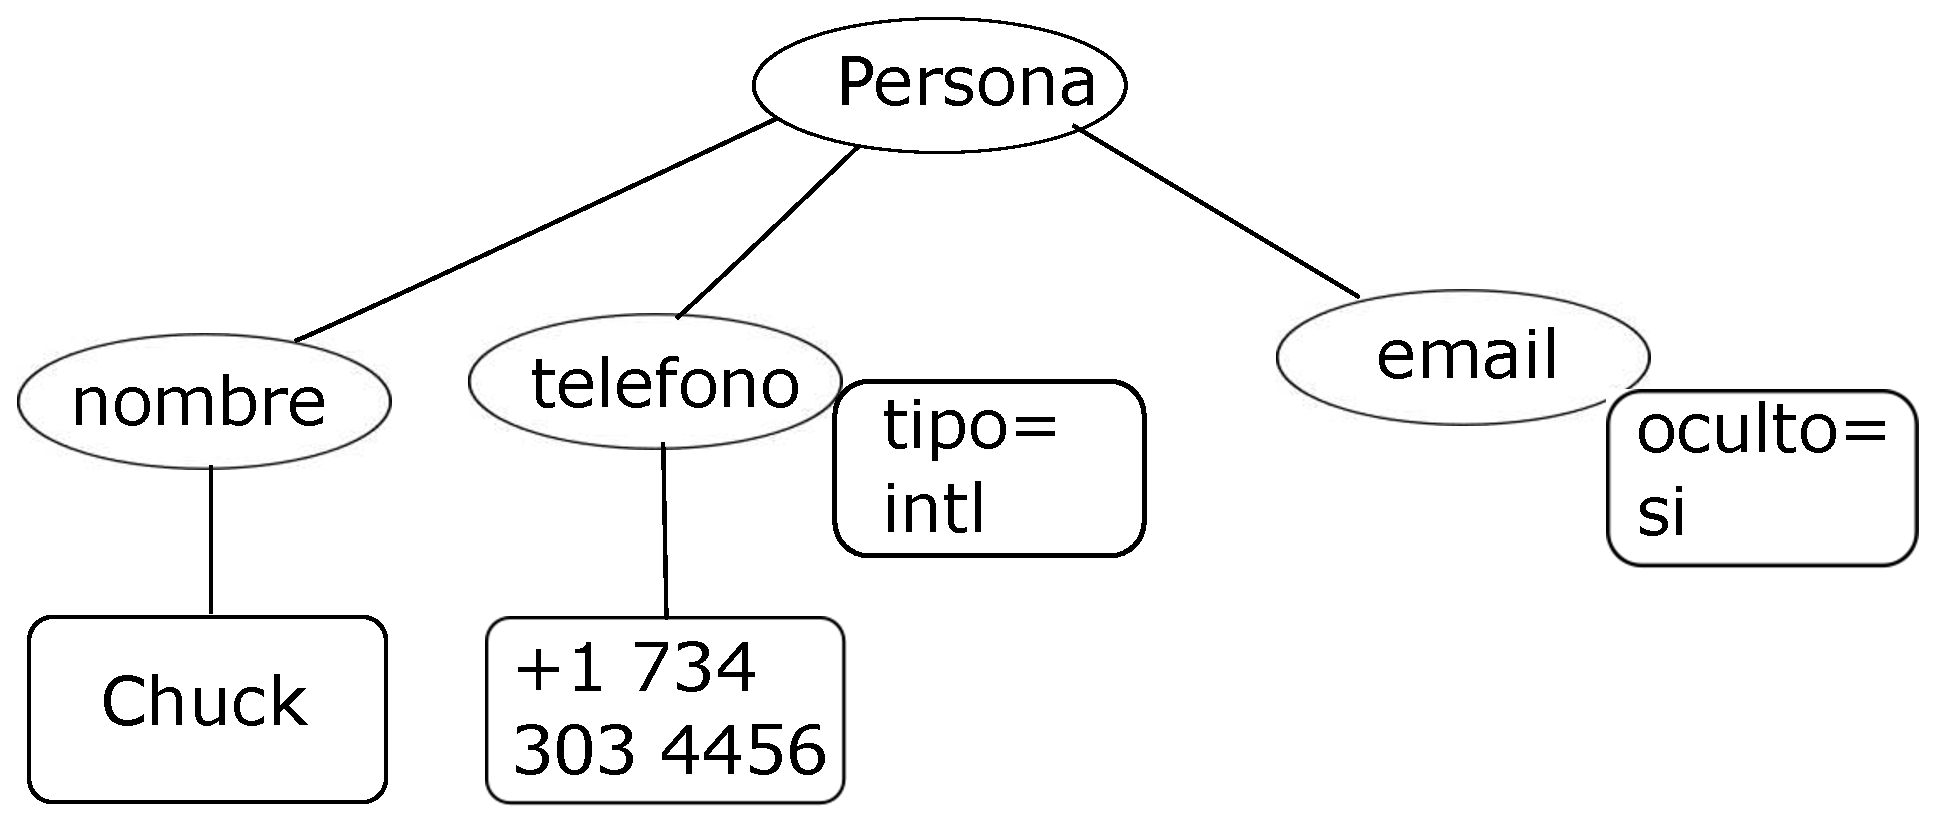
\includegraphics[height=1.50in]{figs2/xml-tree.eps}}
\afterfig

\section{Análisis de XML}

\index{ElementTree}
\index{ElementTree!fromstring}
\index{ElementTree!find}
He aquí una aplicación sencilla que analiza el XML anterior
y extrae algunos elementos de él:

\beforeverb
\begin{verbatim}
import xml.etree.ElementTree as ET

datos = '''
<persona>
  <nombre>Chuck</nombre>
  <telefono tipo="intl">
     +1 734 303 4456
   </telefono>
   <email oculto="si"/>
</persona>'''

arbol = ET.fromstring(datos)
print 'Nombre:',arbol.find('nombre').text
print 'Attr:',arbol.find('email').get('oculto')
\end{verbatim}
\afterverb
%
La llamada a {\tt fromstring} convierte la representación de cadena
del XML en un ``árbol'' de nodos XML. Una vez tenemos el XML
como un árbol, disponemos de una serie de métodos que podemos llamar para
extraer porciones de datos de ese XML.

La función {\tt find} busca a través del árbol XML
y recupera un {\bf nodo} que coincide con la etiqueta especificada.
Cada nodo tiene cierto texto, ciertos atributos (como en este caso ``oculto''), y
ciertos nodos ``hijos''. Cada nodo puede ser el origen de otro árbol de nodos.

\beforeverb
\begin{verbatim}
Nombre: Chuck
Attr: si
\end{verbatim}
\afterverb
%
El usar un analizador de XML como {\tt ElementTree} tiene la ventaja
de que, a pesar de que el XML de este ejemplo es bastante sencillo, resulta
que hay un montón de reglas respecto a la validez del XML, y el uso de
{\tt ElementTree} nos permite extraer datos del XML sin
preocuparnos acerca de esas reglas de sintaxis.

\section{Desplazamiento a través de los nodos}

\index{ElementTree!findall}
\index{ElementTree!get}
A menudo el XML tiene múltiples nodos y tenemos que escribir un bucle
para procesarlos todos. En el programa siguiente,
usamos un bucle para recorrer todos los nodos {\tt usuario}:

\beforeverb
\begin{verbatim}
import xml.etree.ElementTree as ET

entrada = '''
<cosa>
    <usuarios>
        <usuario x="2">
            <id>001</id>
            <nombre>Chuck</nombre>
        </usuario>
        <usuario x="7">
            <id>009</id>
            <nombre>Brent</nombre>
        </usuario>
    </usuarios>
</cosa>'''

cosa = ET.fromstring(entrada)
lst = cosa.findall('usuarios/usuario')
print 'Cantidad de usuarios:', len(lst)

for elemento in lst:
    print 'Nombre', elemento.find('nombre').text
    print 'Id', elemento.find('id').text
    print 'Atributo', elemento.get('x')
\end{verbatim}
\afterverb
%
El método {\tt findall} devuelve a Python una lista de subárboles que
representan las estructuras {\tt usuario} del árbol XML. A continuación podemos
escribir un bucle {\tt for} que busque en cada uno de los nodos usuario,
e imprima el texto de los elementos {\tt nombre} e {\tt id}, además del
atributo {\tt x} de cada nodo {\tt usuario}.

\beforeverb
\begin{verbatim}
Cantidad de usuarios: 2
Nombre Chuck
Id 001
Atributo 2
Nombre Brent
Id 009
Atributo 7
\end{verbatim}
\afterverb
%

\section{JavaScript Object Notation - JSON}
\index{JSON}
\index{JavaScript Object Notation}

El formato JSON se inspiró en el formato de objetos y arrays que se usa en el lenguaje
JavaScript. Pero como Python se inventó antes que JavaScript, la sintaxis usada en Python
para los diccionarios y listas influyeron la sintaxis de JSON. De modo que el formato
del JSON es casi idéntico a la combinación de listas y diccionarios de Python.

He aquí una codificación JSON que es más o menos equivalente al XML del ejemplo anterior:

\beforeverb
\begin{verbatim}
{
  "nombre" : "Chuck",
  "telefono" : {
    "tipo" : "intl",
    "numero" : "+1 734 303 4456"
   },
   "email" : {
     "oculto" : "si"
   }
}
\end{verbatim}
\afterverb
%
Si te fijas encontrarás ciertas diferencias. La primera, en XML se pueden añadir atributos como
``intl'' a la etiqueta ``telefono''. En JSON, simplemente tenemos parejas clave-valor.
Además, la etiqueta ``persona'' de XML ha desaparecido, reemplazada por un conjunto
de llaves exteriores.

En general, las estructuras JSON son más simples que las de XML, debido a que JSON tiene
menos capacidades. Pero JSON tiene la ventaja de que mapea {\em directamente} hacia una
combinación de diccionarios y listas. Y dado que casi todos los lenguajes de programación
tienen algo equivalente a los diccionarios y listas de Python, JSON es un formato
muy intuitivo para que dos programas que vayan a cooperar intercambien datos.

JSON se está convirtiendo rápidamente en el formato elegido para casi todos los intercambios
de datos entre aplicaciones, debido a su relativa simplicidad comparado con XML.

\section{Análisis de JSON}

El JSON se construye anidando diccionarios (objetos) y listas según se necesite.
En este ejemplo, vamos a representar una lista de usuarios en la cual cada usuario es un
conjunto de parejas clave-valor (es decir, un diccionario). De modo que tendremos una lista
de diccionarios.

En el programa siguiente, usaremos la librería integrada {\bf json} para analizar
el JSON y leer los datos. Compáralo cuidadosamente con los datos y código XML
equivalentes que usamos antes. El JSON tiene menos detalles, de modo que podemos saber de
antemano que vamos a obtener una lista y que la lista es de usuarios y además que cada usuario es un
conjunto de parejas clave-valor. El JSON es más escueto (una ventaja), pero también es
menos auto-descriptivo (una desventaja).

\beforeverb
\begin{verbatim}
import json

entrada = '''
[
  { "id" : "001",
    "x" : "2",
    "nombre" : "Chuck"
  } ,
  { "id" : "009",
    "x" : "7",
    "nombre" : "Brent"
  } 
]'''

info = json.loads(entrada)
print 'Cantidad de usuarios:', len(info)

for elemento in info:
    print 'Nombre', elemento['nombre']
    print 'Id', elemento['id']
    print 'Atributo', elemento['x']
\end{verbatim}
\afterverb
%
Si comparas el código que extrae los datos del JSON y XML analizado,
verás que lo que obtenemos de {\bf json.loads()} es una lista de Python
que recorreremos con un bucle {\tt for}, y cada elemento dentro de esa lista
es un diccionario de Python. Una vez analizado el JSON, podemos usar el operador
índice de Python para extraer los distintos fragmentos de datos de cada usuario. No
tenemos que usar la librería JSON para rebuscar a través del JSON analizado, ya que los
datos devueltos son simplemente estructuras nativas de Python.

La salida de este programa es exactamente la misma que la de la versión XML anterior.

\beforeverb
\begin{verbatim}
Cantidad de usuarios: 2
Nombre Chuck
Id 001
Atributo 2
Nombre Brent
Id 009
Atributo 7
\end{verbatim}
\afterverb
%
En general, hay una tendencia en la industria a apartarse del XML y pasar al JSON para
los servicios web. Debido a que JSON es más sencillo, y se mapea de forma más directa hacia
estructuras de datos nativas que ya tenemos en los lenguajes de programación, el código de
análisis y extracción de datos normalmente es más sencillo y directo usando JSON.
Pero XML es más auto-descriptivo, y por eso hay ciertas
aplicaciones en las cuales XML mantiene su ventaja. Por ejemplo, la mayoría de los
procesadores de texto almacenan sus documentos internamente usando XML en vez de JSON.

\section{Interfaces de programación de aplicaciones}

Ahora ya tenemos la capacidad de intercambiar datos entre aplicaciones usando el Protocolo
de Transporte de Hipertexto (HTTP), y un modo de representar estructuras de datos complejas
para poder enviar y recibir los datos entre esas aplicaciones, a través del eXtensible 
Markup Language (XML) o del JavaScript Object Notation (JSON).

El paso siguiente consiste en empezar a definir y documentar ``contratos'' entre
aplicaciones usando estas técnicas. El nombre corriente para estos
contratos entre aplicaciones es {\bf Interfaces de Programación
de Aplicaciones}, o APIs. Cuando se utiliza una API, normalmente un programa
crea un conjunto de {\bf servicios} disponibles para que los usen otras aplicaciones
y publica las APIs (es decir, las ``reglas'') que deben ser seguidas para
acceder a los servicios proporcionados por el programa.

Cuando comenzamos a construir programas con funcionalidades que incluyen
el acceso a servicios proporcionados por otros,
se utiliza un planteamiento llamado {\bf Arquitectura Orientada a Servicios}, o SOA, por sus
iniciales en inglés.
Un planteamiento SOA es aquel en el cual nuestra aplicación principal usa los servicios
de otras aplicaciones. Un planteamiento no-SOA es aquel en el cual tenemos
una única aplicación independiente que contiene ella misma todo el código
necesario para su implementación.

Podemos encontrar multitud de ejemplos de SOAs cuando utilizamos servicios de la web. Podemos ir a un
único sitio web y reservar viajes en avión, hoteles y automóviles, todo ello desde el
mismo sitio. Los datos de los hoteles no están almacenados en los ordenadores de la
compañía aérea. En vez de eso, los ordenadores de la aerolínea contactan con los servicios
de los ordenadores de los hoteles y recuperan los datos de los alojamientos que presentan al
usuario. Cuando el usuario acepta realizar una reserva de un hotel usando el sitio web
de una aerolínea, ésta utiliza otro servicio web en los sistemas de los hoteles para realizar
la reserva real. Y cuando llega el momento de cargar en tu tarjeta de crédito el importe de la
transacción completa, hay todavía otros ordenadores diferentes involucrados en el proceso.

\beforefig
\centerline{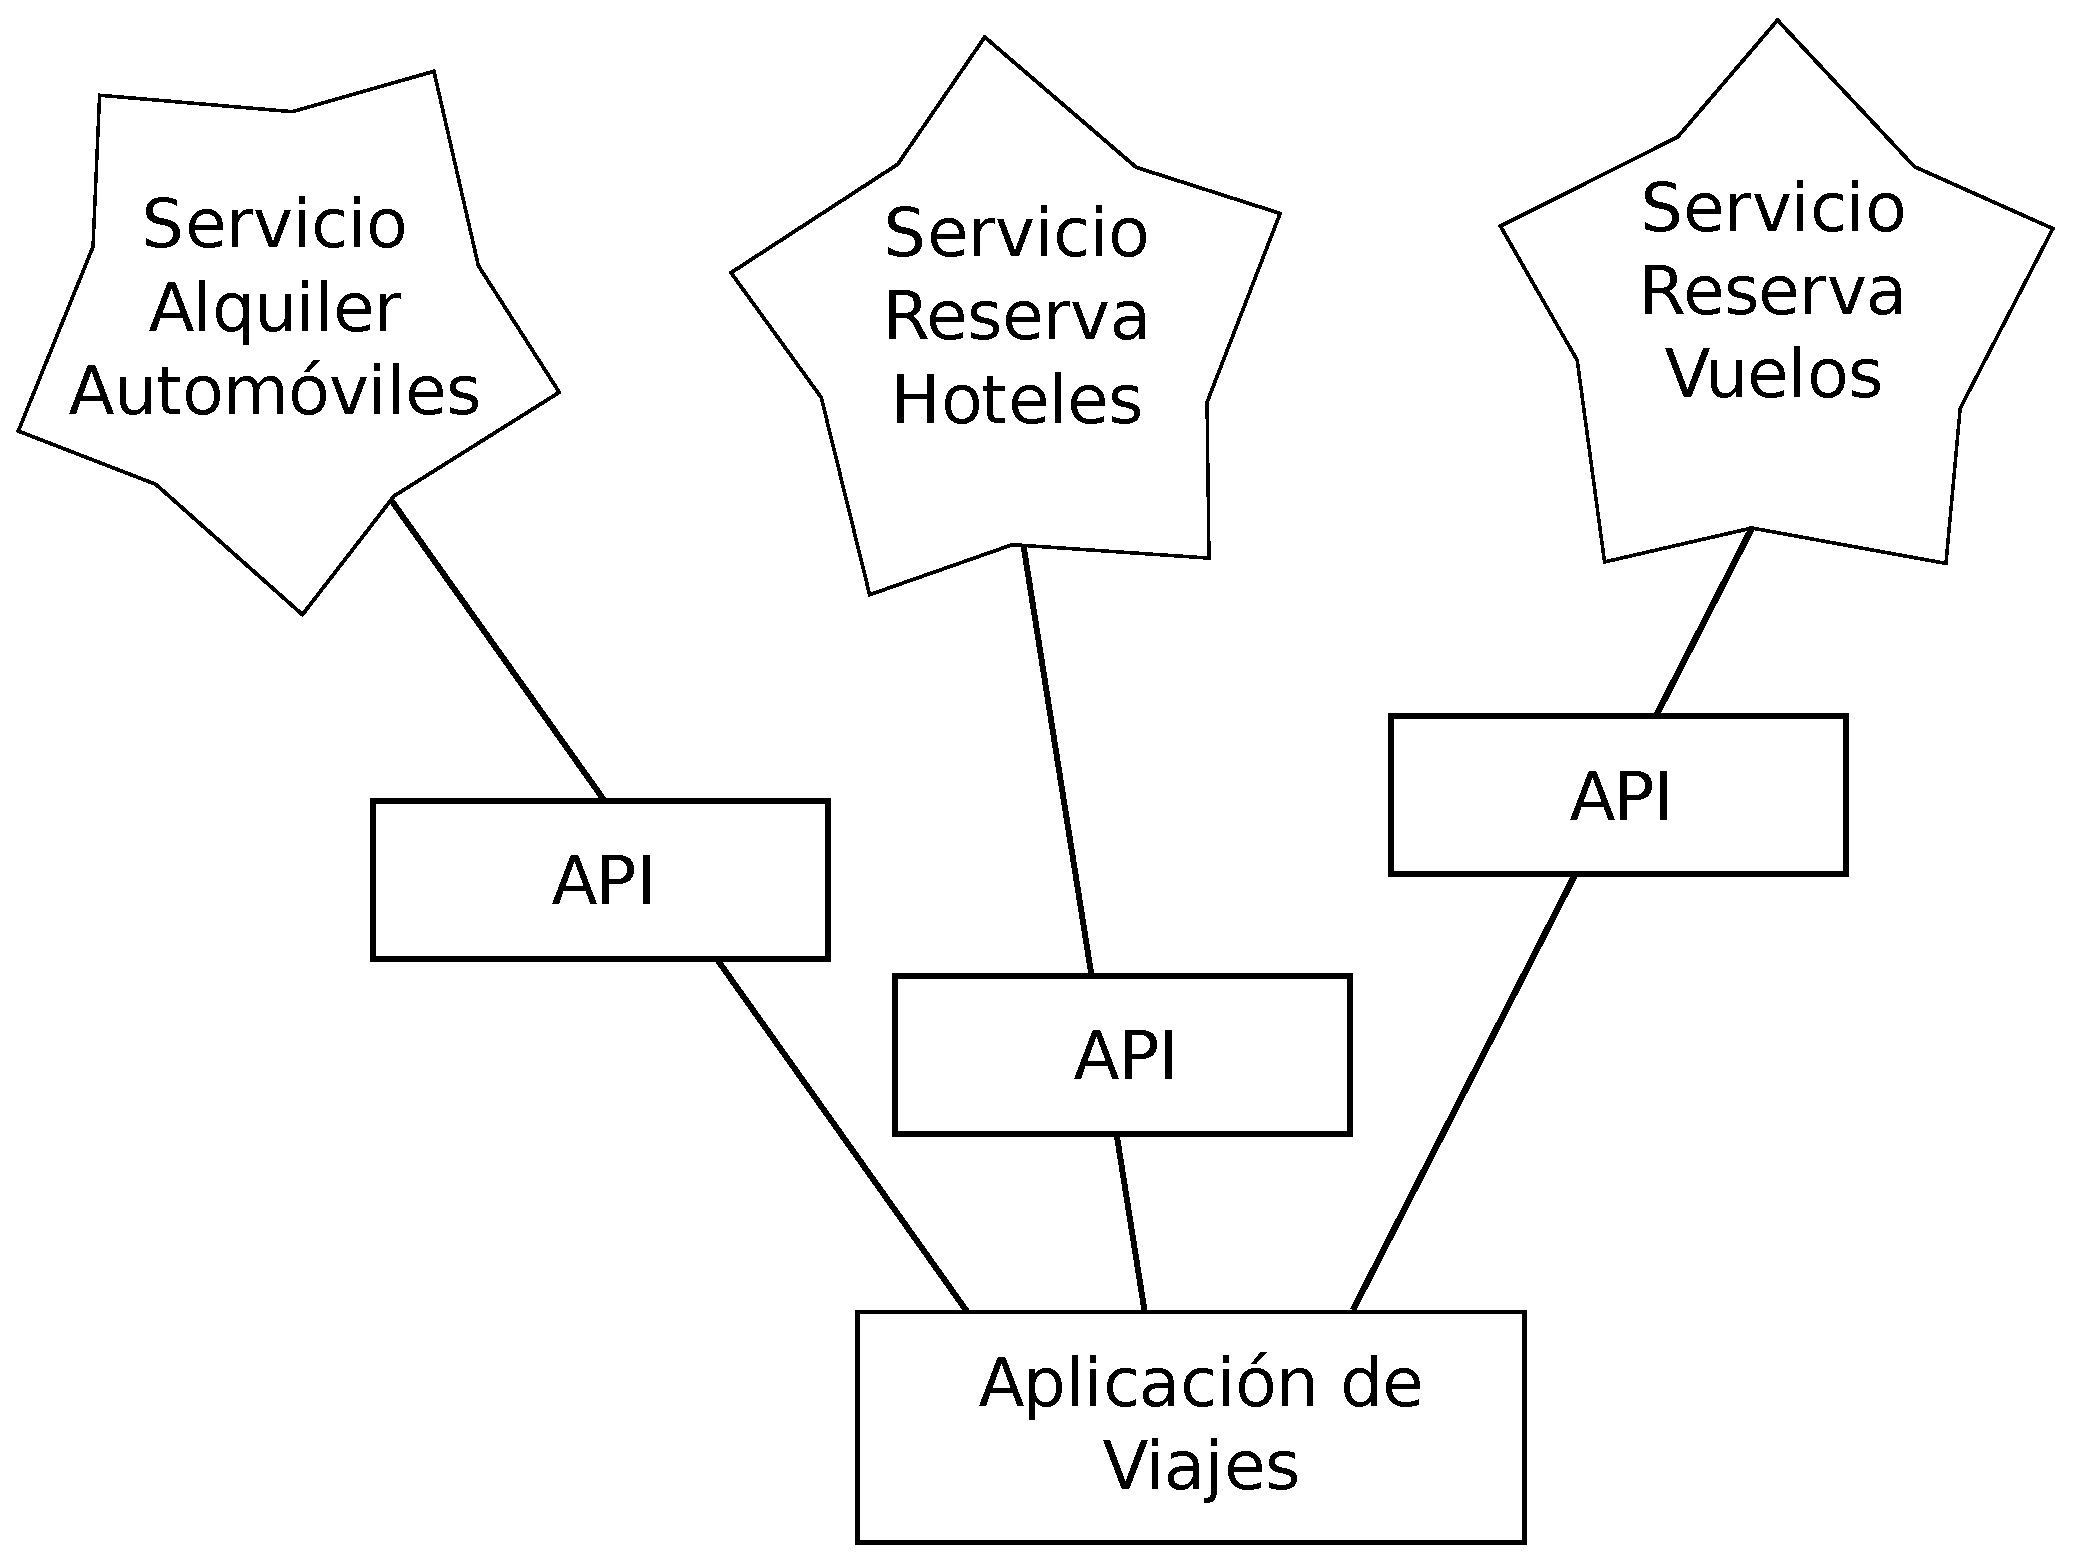
\includegraphics[height=2.50in]{figs2/soa.eps}}
\afterfig

Una Arquitectura Orientada a Servicios tiene muchas ventajas, que incluyen: (1)
siempre se mantiene una única copia de los datos (lo cual resulta particularmente
importante en ciertas cosas como las reservas hoteleras, las cuales no se pueden duplicar)
y (2) los propietarios de los datos pueden imponer las reglas acerca del uso de esos datos.
Con estas ventajas, un sistema SOA debe ser diseñado con mucho cuidado para
tener buen rendimiento y satisfacer las necesidades de los usuarios.

Cuando una aplicación ofrece un conjunto de servicios en su API disponibles a través de la
web, éstos reciben el nombre de {\bf servicios web}.

\section{Servicio web de geocodificación de Google}
\index{Google}
\index{geocoding}
\index{web service}

Google tiene un servicio web excelente que nos permite hacer uso de su
enorme base de datos de información geográfica. Podemos enviar una cadena de búsqueda
geográfica, como ``Ann Arbor, MI'' a su API de geocodificación y conseguir que Google
nos devuelva la situación en un mapa de dónde podría estar nuestra cadena de
búsqueda, además de los puntos de referencia en los alrededores.

El servicio de geocodificación es gratuito pero limitado, de modo que no se puede hacer
un uso intensivo de esta API en una aplicación comercial. Pero si tienes ciertos datos
estadísticos en los cuales un usuario final ha introducido una localización en formato
libre en un cuadro de texto, puedes usar esta API para limpiar esos datos de forma
bastante efectiva.

{\em Cuando se usa una API libre, como la API de geocodificación de Google, se debe ser
respetuoso con el uso de los recursos. Si hay demasiada gente que abusa de ello,
Google puede interrumpir o restringir significativamente su servicio gratuito.}
\index{rate limiting}

Puedes leer la documentación online de este servicio, pero es bastante sencillo
y puedes incluso probarlo desde un navegador, simplemente tecleando la siguiente URL
en él:

\url{http://maps.googleapis.com/maps/api/geocode/json?sensor=false &address=Ann+Arbor%2C+MI}

Asegúrate de limpiar la URL y eliminar cualquier espacio de ella antes de pegarla
en el navegador.

La siguiente es una aplicación sencilla que pide al usuario una cadena de búsqueda,
llama a la API de geocodificación de Google y extrae información del JSON que nos devuelve.

\beforeverb
\begin{verbatim}
import urllib
import json

urlservicio = 'http://maps.googleapis.com/maps/api/geocode/json?'

while True:
    direccion = raw_input('Introduce ubicación: ')
    if len(direccion) < 1 : break

    url = urlservicio + urllib.urlencode({'sensor':'false', 
          'address': direccion})
    print 'Recuperando', url
    uh = urllib.urlopen(url)
    datos = uh.read()
    print 'Recibidos',len(datos),'caracteres'

    try: js = json.loads(str(datos))
    except: js = None
    if 'status' not in js or js['status'] != 'OK':
        print '==== Fallo de Recuperación ===='
        print datos
        continue

    print json.dumps(js, indent=4)

    lat = js["results"][0]["geometry"]["location"]["lat"]
    lng = js["results"][0]["geometry"]["location"]["lng"]
    print 'lat',lat,'lng',lng
    ubicacion = js['results'][0]['formatted_address']
    print ubicacion
\end{verbatim}
\afterverb
%
El programa toma la cadena de búsqueda y construye una URL
codificándola como parámetro dentro de ella, utilizando luego
{\bf urllib} para recuperar el texto de la API de geocodificación de Google.
A diferencia de una página web estática, los datos que obtenemos dependen de los
parámetros que enviemos y de los datos geográficos almacenados en los servidores de Google.

Una vez recuperados los datos JSON, los analizamos con la librería
{\bf json} y realizamos unas pequeñas comprobaciones para asegurarnos de que hemos recibido
datos válidos. Finalmente, extraemos la información que estábamos buscando.

La salida del programa es la siguiente (parte del JSON recibido
ha sido eliminado):

\beforeverb
\begin{verbatim}
$ python geojson.py
Introduce ubicación: Ann Arbor, MI
Recuperando http://maps.googleapis.com/maps/api/
  geocode/json?sensor=false&address=Ann+Arbor%2C+MI
Recibidos 1669 caracteres
{
    "status": "OK", 
    "results": [
        {
            "geometry": {
                "location_type": "APPROXIMATE", 
                "location": {
                    "lat": 42.2808256, 
                    "lng": -83.7430378
                }
            }, 
            "address_components": [
                {
                    "long_name": "Ann Arbor", 
                    "types": [
                        "locality", 
                        "political"
                    ], 
                    "short_name": "Ann Arbor"
                } 
            ], 
            "formatted_address": "Ann Arbor, MI, USA", 
            "types": [
                "locality", 
                "political"
            ]
        }
    ]
}
lat 42.2808256 lng -83.7430378
Ann Arbor, MI, USA
Introduce ubicación:
\end{verbatim}
\afterverb
%
Puedes descargar
\url{www.py4inf.com/code/geojson.py} y
\url{www.py4inf.com/code/geoxml.py} para revisar
las variantes JSON y XML de la API de geocodificación de Google.

\section{Seguridad y uso de APIs}
\index{OAuth}
\index{API!key}

Resulta bastante frecuente que se necesite algún tipo de
``clave API'' para hacer uso de una API comercial. La
idea general es que ellos quieren saber quién está usando
sus servicios y cuánto los utiliza cada usuario.
Tal vez tienen distintos niveles (gratuitos y de pago) de sus servicios,
o una política que limita el número de peticiones
que un único usuario puede realizar durante un determinado
periodo de tiempo.

A veces, una vez que tienes tu clave API, tan sólo debes incluirla
como parte de los datos POST, o tal vez como parámetro
dentro de la URL que usas para llamar a la API.

Otras veces, el vendedor quiere aumentar la seguridad del
origen de las peticiones, de modo que además espera que
envíes mensajes firmados criptográficamente, usando claves
compartidas y secretas. Una tecnología muy habitual que se utiliza
para firmar peticiones en Internet se llama {\bf OAuth}.
Puedes leer más acerca del protocolo OAuth en 
\url{http://www.oauth.net}.

A medida que la API de Twitter ha ido haciéndose más valiosa, Twitter
ha pasado de una API abierta y pública a una API que necesita
el uso de firmas OAuth en cada solicitud. Afortunadamente,
aún hay unas cuantas librerías OAuth buenas y gratuitas,
de modo que te puedes ahorrar el tener que escribir una implementación OAuth
desde cero leyendo las especificaciones. Estas librerías tienen
una complejidad variable y varios niveles distintos en cuanto a variedad de características.
El sitio web OAuth tiene información sobre varias librerías OAuth.

Para el programa de ejemplo siguiente, descargaremos los ficheros
{\bf twurl.py}, {\bf hidden.py}, 
{\bf oauth.py}, 
y
{\bf twitter1.py} desde
\url{www.py4inf.com/code}, y los pondremos todos juntos en una carpeta
de tu ordenador.

Para usar estos programas debes tener una cuenta de Twitter,
y autorizar a tu código Python como aplicación permitida,
estableciendo diversos parámetros (key, secret, token y token secret). Debes editar
el archivo {\bf hidden.py} y colocar esas cuatro cadenas en las
variables apropiadas dentro del fichero:

\beforeverb
\begin{verbatim}
    def auth() :
        return { "consumer_key" : "h7L...GNg",
            "consumer_secret" : "dNK...7Q",
            "token_key" : "101...GI",
            "token_secret" : "H0yM...Bo" }
\end{verbatim}
\afterverb
%
El servicio web de Twitter es accesible usando una URL como esta:

\url{https://api.twitter.com/1.1/statuses/user_timeline.json}

Pero una vez que se ha añadido toda la información de seguridad, la URL
se parecerá más a esto:

\beforeverb
\begin{verbatim}
https://api.twitter.com/1.1/statuses/user_timeline.json?count=2
&oauth_version=1.0&oauth_token=101...SGI&screen_name=drchuck
&oauth_nonce=09239679&oauth_timestamp=1380395644
&oauth_signature=rLK...BoD&oauth_consumer_key=h7Lu...GNg
&oauth_signature_method=HMAC-SHA1
\end{verbatim}
\afterverb
%
Puedes leer la especificación OAuth si quieres saber más
acerca del significado de los distintos parámetros que
hemos añadido para cumplir con los requerimientos de seguridad de OAuth.

Para los programas que ejecutamos con Twitter, ocultamos toda la
complejidad dentro de los archivos {\bf oauth.py} y {\bf twurl.py}.
Simplemente ajustamos los parámetros secretos en {\bf hidden.py}, luego
enviamos la URL deseada a la función {\bf twurl.augment()}
y el código de la librería añade todos los parámetros
necesarios a la URL por nosotros.

Este programa ({\bf twitter1.py}) recupera la línea de tiempo
de un usuario de Twitter concreto y nos la devuelve en formato
JSON como una cadena. Vamos a imprimir simplemente los primeros 250
caracteres de esa cadena:

\beforeverb
\begin{verbatim}
import urllib
import twurl

TWITTER_URL='https://api.twitter.com/1.1/statuses/user_timeline.json'

while True:
    print ''
    cuenta = raw_input('Introduce Cuenta de Twitter:')
    if ( len(cuenta) < 1 ) : break
    url = twurl.augment(TWITTER_URL,
        {'screen_name': cuenta, 'count': '2'} )
    print 'Recuperando', url
    conexion = urllib.urlopen(url)
    datos = conexion.read()
    print datos[:250]
    cabeceras = conexion.info().dict
    # print cabeceras
    print 'Restante', cabeceras['x-rate-limit-remaining']
\end{verbatim}
\afterverb
%
Cuando el programa se ejecuta, produce la salida siguiente: 
 
\beforeverb
\begin{verbatim}
Introduce Cuenta de Twitter:drchuck
Recuperando https://api.twitter.com/1.1/ ...
[{"created_at":"Sat Sep 28 17:30:25 +0000 2013","
id":384007200990982144,"id_str":"384007200990982144",
"text":"RT @fixpert: See how the Dutch handle traffic 
intersections: http:\/\/t.co\/tIiVWtEhj4\n#brilliant",
"source":"web","truncated":false,"in_rep
Restante 178

Introduce Cuenta de Twitter:fixpert
Recuperando https://api.twitter.com/1.1/ ...
[{"created_at":"Sat Sep 28 18:03:56 +0000 2013",
"id":384015634108919808,"id_str":"384015634108919808",
"text":"3 months after my freak bocce ball accident, 
my wedding ring fits again! :)\n\nhttps:\/\/t.co\/2XmHPx7kgX",
"source":"web","truncated":false,
Restante 177

Introduce Cuenta de Twitter:
\end{verbatim}
\afterverb
%
Junto con los datos de la línea del tiempo, Twitter también devuelve
metadatos sobre la petición en las cabeceras de respuesta HTTP.
Una cabecera en particular, {\bf x-rate-limit-remaining}, nos informa
sobre cuántas peticiones podemos hacer antes de que seamos bloqueados
por un corto periodo de tiempo. Puedes ver cómo cada vez que realizamos
una petición a la API nuestros intentos restantes van disminuyendo.

En el ejemplo siguiente, recuperamos los amigos de un usuario en Twitter,
analizamos el JSON devuelto y extraemos parte de la información
sobre esos amigos. También vaciamos el JSON después de analizarlo e
``imprimirlo ordenado'', con un justificado de cuatro caracteres para permitirnos
estudiar minuciosamente los datos cuando queramos extraer más campos.

\beforeverb
\begin{verbatim}
import urllib
import twurl
import json

TWITTER_URL = 'https://api.twitter.com/1.1/friends/list.json'

while True:
    print ''
    cuenta = raw_input('Introduce Cuenta de Twitter:')
    if ( len(cuenta) < 1 ) : break
    url = twurl.augment(TWITTER_URL,
        {'screen_name': cuenta, 'count': '5'} )
    print 'Recuperando', url
    conexion = urllib.urlopen(url)
    datos = conexion.read()
    cabeceras = conexion.info().dict
    print 'Restantes', cabeceras['x-rate-limit-remaining']
    js = json.loads(datos)
    print json.dumps(js, indent=4)

    for u in js['users'] :
        print u['screen_name']
        s = u['status']['text']
        print '  ',s[:50]
\end{verbatim}
\afterverb
%
Dado que el JSON se transforma en un conjunto de listas y diccionarios de Python,
podemos usar una combinación del operador índice junto con bucles {\tt for} para
movernos a través de las estructuras de datos devueltas con muy poco
código Python.

La salida del programa se parece a la siguiente (parte de los datos
se han acortado para que quepa en la página):

\beforeverb
\begin{verbatim}
Introduce Cuenta de Twitter:drchuck
Recuperando https://api.twitter.com/1.1/friends ...
Restantes 14
{
    "next_cursor": 1444171224491980205, 
    "users": [
        {
            "id": 662433, 
            "followers_count": 28725, 
            "status": {
                "text": "@jazzychad I just bought one .__.", 
                "created_at": "Fri Sep 20 08:36:34 +0000 2013", 
                "retweeted": false, 
            }, 
            "location": "San Francisco, California", 
            "screen_name": "leahculver", 
            "name": "Leah Culver", 
        }, 
        {
            "id": 40426722, 
            "followers_count": 2635, 
            "status": {
                "text": "RT @WSJ: Big employers like Google ...", 
                "created_at": "Sat Sep 28 19:36:37 +0000 2013", 
            }, 
            "location": "Victoria Canada", 
            "screen_name": "_valeriei", 
            "name": "Valerie Irvine", 
    ], 
    "next_cursor_str": "1444171224491980205"
}
leahculver
   @jazzychad I just bought one .__.
_valeriei
   RT @WSJ: Big employers like Google, AT&amp;T are h
ericbollens
   RT @lukew: sneak peek: my LONG take on the good &a
halherzog
   Learning Objects is 10. We had a cake with the LO,
scweeker
   @DeviceLabDC love it! Now where so I get that "etc

Introduce Cuenta de Twitter:
\end{verbatim}
\afterverb
%
El último trozo de la salida es donde podemos ver cómo el bucle for lee los
cinco ``amigos'' más recientes de la cuenta de Twitter del {\bf drchuck}
e imprime el estado más reciente de cada uno de ellos. Hay
muchos más datos disponibles en el JSON devuelto. Si miras
la salida del programa, podrás ver que el ``encuentra a los amigos''
de una cuenta particular tiene una limitación de usos distinta al
número de consultas de líneas del tiempo que está permitido realizar en un periodo de tiempo.

Estas claves de seguridad de la API permiten a Twitter tener la certeza de que
sabe quién está usando su API y datos y a qué nivel. El enfoque del
límite de usos nos permite hacer captaciones de datos sencillas e individuales, pero
no nos permite crear un producto que extraiga datos de esa API
millones de veces al día.

\section{Glosario}

\begin{description}

\item[API:] Interfaz de Programación de Aplicaciones - Un contrato entre
aplicaciones que define los patrones de interacción entre
los componentes de dos aplicaciones.
\index{API}

\item[Árbol de elementos:] Una librería integrada de Python que se utiliza
para analizar datos XML.
\index{ElementTree}

\item[JSON:] Notación de Objetos JavaScript. Un formato que permite
el marcado de estructuras de datos basadas en la sintaxis de los Objetos
JavaScript.
\index{JSON}
\index{JavaScript Object Notation}

\item[SOA:] Arquitectura Orientada a Servicios. Cuando una aplicación
está formada por componentes conectados a través de una red.
\index{SOA}
\index{Service Oriented Architecture}

\item[XML:] Lenguaje de Marcas eXtensible. Un formato que permite
el marcado de datos estructurados.
\index{XML}
\index{eXtensible Markup Language}

\end{description}

\section{Ejercicios}

\begin{ex}
Cambia bien el programa
\url{www.py4inf.com/code/geojson.py} o bien
\url{www.py4inf.com/code/geoxml.py} para imprimir en pantalla el
código de país de dos caracteres de los datos recuperados.
Añade comprobación de errores, de modo que tu programa no rastree esos datos
si el código del país no está presente. Una vez que lo tengas
funcionando, busca ``Océano Atlántico'' y asegúrate
de que es capaz de gestionar ubicaciones que no están dentro de ningún país.
\end{ex}
